\documentclass[titlepage=firstiscover, bibliography=totoc, captions=tableheading]{scrartcl}
\title{V207: Das Kugelfall - Viskometer nach Höppler}
\author{
  Simon Schulte
  \texorpdfstring{
    \\
    \href{mailto:simon.schulte@udo.edu}{simon.schulte@udo.edu}
  }{}
  \texorpdfstring{\and}{, }
  Tim Sedlaczek
  \texorpdfstring{
    \\
    \href{mailto:tim.sedlaczek@udo.edu}{tim.sedlaczek@udo.edu}
  }{}
}
\publishers{TU Dortmund – Fakultät Physik}

\date{Durchführung: 15.11.2016\\
      Abgabe: xx.11.2016}

\usepackage[aux]{rerunfilecheck}
\usepackage{polyglossia}
\setmainlanguage{german}
\usepackage{amsmath}
\usepackage{amssymb}
\usepackage{mathtools}
\usepackage{fontspec}

\usepackage{scrhack}
\usepackage{float}
\floatplacement{table}{htbp}
\floatplacement{figure}{htbp}

\usepackage[locale=DE, separate-uncertainty=true, per-mode=symbol-or-fraction]{siunitx}
%\usepackage{siunitx}

\usepackage[style=alphabetic]{biblatex}
\addbibresource{lit.bib}

\usepackage[section, below]{placeins}
\usepackage[labelfont=bf,
font=small,
width=0.9\textwidth,
format=plain,
indention=1em]{caption}
\usepackage{graphicx}
\usepackage{grffile}
\usepackage{subcaption}

\usepackage[math-style=ISO, bold-style=ISO, sans-style=italic, nabla=upright, partial=upright]{unicode-math}
\setmathfont{Latin Modern Math}

\usepackage[autostyle]{csquotes}

\usepackage[unicode]{hyperref}

\usepackage{bookmark}

\usepackage{booktabs}

\begin{document}

\maketitle
\thispagestyle{empty}
\tableofcontents
\newpage
\section{Zielsetzung}
\label{sec:zielsetzung}
Es soll mit Hilfe der Kugelfallmethode bei einer laminaren Strömung die
Temperaturabhängigkeit der dynamischen Viskosität von destilliertem Wasser
bestimmt werden.
\section{Theorie}
\label{sec:theorie}
Wenn ein Körper sich durch eine Flüssigkeit bewegt, wirken, in entgegengesetzter
Richtung zur Gravitation Reibungskräfte. Diese hängen von der Fläche A, der Geschwindigkeit v
des Körpers und von der Viskosität $\eta$ der Flüssigkeit ab. Die Viskosität
einer Flüssigkeit hängt von der Temperatur ab. In diesem Versuch wird die
Viskosität von destilliertem Wasser untersucht, welche mit zunehmender
Temperatur geringer wird. Um besagte Viskosität zu bestimmen, lässt man eine
Kugel mit Radius $r$ laminar durch ein mit destilliertem Wasser gefülltes Rohr
fallen. Die Stokesche Reibung wird dann mit der Formel
\begin{equation}
  F_R = 6 \pi \eta v r
\end{equation}
bestimmt, wobei $v$ die Fallgeschwindigkeit ist. Die Reibungskraft $\vec{F_R}$
und die Antriebskraft $\vec{F_A}$ wirken dabei der Gravitationskraft $\vec{F_g}$
entgegen. Die beiden entgegengesetzten Kräfte werden stärker, umso schneller
der Körper sich bewegt, solange, bis ein Kräftegleichgewicht entsteht und der
Körper eine konstante Geschwindigkeit erreicht. Dabei wird eine annäherend
laminare Strömung erzeugt. Indem man die Reynoldsche Zahl für die Bewegung
errechnet, lässt sich dann sagen, ob die Bewegung des Körpers tatsächlich
laminar war. Es gibt eine kritische Zahl für destilliertes Wasser, anhand
welcher man sehen kann, wenn die errechnete Reynoldsche Zahl kleiner oder größer
ist, ob die Bewegung laminar oder turbulent war. Um eine laminare Bewegung zu
gewährleisten, wird das Fallrohr um wenige Grade geneigt, sodass die Kugel an der
Rohrwand hinabgleitet und sich keine Wirbel ausbilden können. Der Durchmesser
des Körpers selbst ist nur geringfügig geringer, als der des Rohres. Mithilfe
der Dichte des destillierten Wassers $\rho_{Fl}$, der Dichte des Körpers $\rho_K$,
der Apperaturkonstante $K$ und der Fallzeit $t$ lässt sich dann die Viskosität
$\eta$ berechnen:
\begin{equation}
  \eta = K (\rho_K - \rho_{Fl}) \cdot t
\end{equation}
Dabei enthält die Apperaturkonstante $K$ sowohl die Kugelgeometrie, als auch
die Fallhöhe. Da die Viskosität von vielen Flüssigkeiten stark
temperaturabhängig ist, wird die temperaturabhängige Viskosität durch die
Andradesche Gleichung:
\begin{equation}
  \eta(T) = A exp (\frac{B}{T})
\end{equation}
beschrieben, mit den Konstanten A und B.

\section{Durchführung}
\label{sec:durchführung}
\subsection{Versuchsaufbau}
Wie in Abbildung 1 gezeigt fällt die Kugel durch ein Rohr, welches mit Wasser
gefüllt ist. Durch zwei Stopfen und jeweils einer Schraube über diesen Stopfen
an den beiden Rohrenden kann man sowohl Wasser, als auch die Kugel selbst, in das
Rohr füllen. An dem Rohr sind drei Messmarken befestigt, die jeweils mit einem
Abstand von 5 cm auseinander liegen. Diese werden zur Zeitmessung genutzt. Die
Libelle wird genutzt, um zu prüfen, ob das Viskosimeter gerade steht. Um die
Temperatur des Wassers im Rohr regulieren zu können, nutzt man ein Thermostat,
an welchem man die Temperatur des Wassers, welches das Rohr in einem
zylinderförmigen Körper umgibt, einstellen kann.
\begin{figure}[htb]
  \centering
  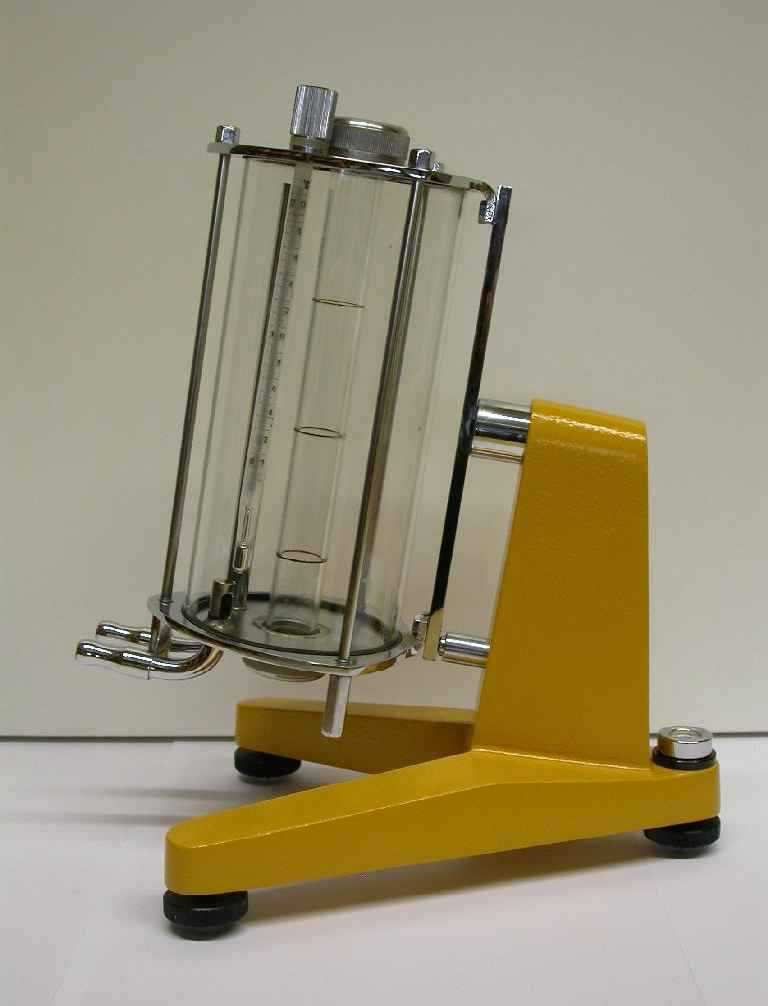
\includegraphics[width=0.5\textwidth]{figure/bild.png}
  \caption{Das Höppler - Viskometer}
  \label{fig:mein_label}
\end{figure}
\subsection{Versuchsdurchführung}
Zunächst bestimmt man die Masse und die geometrischen Maße der beiden Kugeln.
Dabei fällt auf, dass eine Kugel größer als die andere ist.
Daraufhin überprüft man mit Hilfe der Libelle, ob das Viskometer gerade steht.
Als nächstes füllt man das Rohr mit destilliertem Wasser und sorgt dafür, dass sich
möglichst keine Luftbläschen mehr am Rande des Rohres befinden. Dafür nutzt man
einen Glasstab. Dann gibt man vorsichtig die Kugel in das Rohr und achtet
darauf, dass auch an der Kugel möglichst keine Luftbläschen sind, denn diese
würden die Messungen verfälschen. Nun misst man die Zeit, die die beiden Kugeln
bei Zimmertemperatur brauchen, um 10 cm Strecke zurückzulegen, also von der
obersten Markierung zur untersten zu gelangen. Dabei ist auf den bereits in der
Theorie angesprochenen Kräfteausgleich zu achten. Die beiden Markierungen sind
bewusst nicht am oberen Rand des Rohres befestigt, damit die Kugel etwas Zeit
hat, um eine konstante Geschwindigkeit zu erreichen. Durch
das Drehen des Rohres um 180 grad kann man dann die nächste Messung durchführen.
Diese Messung führ man dann für beide Kugeln jeweils 10 mal durch und misst die
Zeit. Für die große Kugel muss dann noch die Apperaturkonstante K bestimmt
werden. Danach heizt man das Wasserbad, welches das Rohr umgibt auf. Man führt
jeweils vier Messungen für 10 verschiedene Temperaturen durch. Diese
befinden sich zwischen 25 und 70 $°C$. Es werden die Zeiten für die größere
Kugel gemessen.
Zuletzt errechnet man die Reynoldsche Zahl für die gemessenen Daten und
überprüft, ob die Strömung laminar ist.
\printbibliography

\end{document}
